%\documentclass[]{beamer}
\documentclass[handout]{beamer}
\usepackage{polski}
\usepackage[utf8]{inputenc}
\usetheme{Warsaw} %motyw 
\usepackage{graphicx}
\usepackage{mathrsfs}
\usepackage{array}
\usepackage{bbm}
\usepackage{multirow}
%\usepackage{wrapfig}
\newtheorem*{definicja}{Definicja}
\newtheorem*{twierdzenie}{Twierdzenie}

\useoutertheme{infolines}
%\useoutertheme{miniframes}

\begin{document}

\author{Paulina Grudzińska}

%\institute{The Faculty of Mathematics and Information Science}
\institute[]
{
Wydział Matematyki i Nauk Informacyjnych\\
Politechniki Warszawskiej 
}
\title{Metoda Optymalizacji Bayesowskiej}
\date{08.07.2019}

\begin{frame} %ramka, nie slajd!!!
\titlepage%strona tytulowa
\vspace{-0.7cm}
\begin{center}
\begin{figure}

\includegraphics[scale=0.25]{logo.png}
\end{figure}
\end{center}
\end{frame}


%%%%%%%%%%%%%%%%%%%%%%%%%%%%%%%%%%%%%%%%%%%%%%

\begin{frame}
\frametitle{Klasyczny problem optymalizacyjny}
\begin{block}{}
Założenia:
\begin{enumerate}
\item $A \subset R^d$,
\item $A$ jest zbiorem wypukłym, 
\item $f$ znana, 
\item $f$ wypukła i różniczkowalna. 
\end{enumerate} 

\end{block}
\pause
\begin{block}{Problem}
Szukamy minimum/maksimum funkcji $f$ w zbiorze $A$.
\end{block}
\end{frame}

\begin{frame}
\frametitle{Metoda Optymalizacji Byesowskiej}
\begin{block}{}
\begin{enumerate}
\item metoda szukania ekstremum funkcji celu kosztownych do szacowania,
\item nie wymaga znajomości postaci funkcji celu, 
\item można ją stosować w przypadku braku założenia wypukłości i istnienia pochodnych, 
\item efektywność MBO wynika z wykorzystania informacji \textit{a priori} do ukierunkowania próbkowania. 
\end{enumerate}
\end{block}
\end{frame}

\begin{frame}
\frametitle{Twierdzenie Bayesa}
\begin{block}{Twierdzenie}
\begin{equation*}
\mathbb{P}(f|D_{1:t}) \propto \mathbb{P} (D_{1:t}|f) \mathbb{P}(f),
\end{equation*}
gdzie: \\
$ $ $x_i$ - i-ta obserwacja, \\
$ $ $f(x_i)$ - wartość funkcji celu w punkcie $x_i$, \\
$ $ $x_{1:t} = \{ x_1, ..., x_t \}$, \\
$ $ $D_{1:t} = \{ x_{1:t}, f(x_{1:t}) \}$,  \\
$ $ $\mathbb{P}(f)$ - informacja \textit{a priori} o funkcji celu.
\end{block}
\end{frame}

\begin{frame}
\frametitle{MBO - algorytm}
\begin{block}{}
\textbf{for} t = 1, 2, . . . \textbf{do} \\
$ $ $ $ Znajdź $x_t = argmax_x \ u(x|D_{1:t-1})$. \\
$ $ $ $ Wyznacz $y_t = f(x_t) + \varepsilon_t$. \\
$ $ $ $ Uaktualnij zbiór danych: $D_{1:t} := \{D_{1:t-1}, (x_t, y_t)\}$. \\
\textbf{end for}
\end{block}
\end{frame}

\begin{frame}
\frametitle{MBO - algorytm}
\begin{center}
\begin{figure}
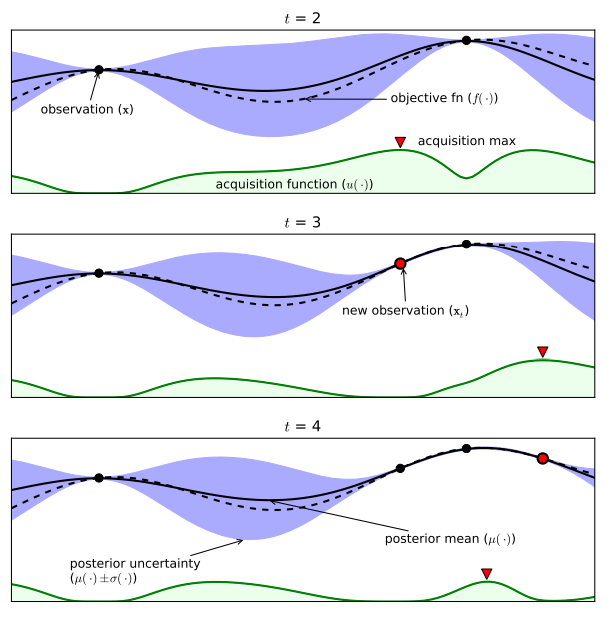
\includegraphics[scale=0.46]{alg.png}
\end{figure}
\end{center}
\end{frame}

\begin{frame}
\frametitle{Funkcja akwizycji \textit{u}}
\begin{center}
\begin{figure}
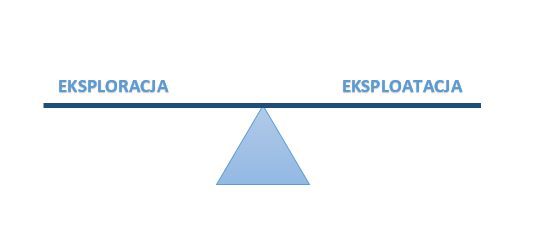
\includegraphics[scale=0.8]{eks.png}
\end{figure}
\end{center}
\end{frame}

\begin{frame}
\frametitle{Funkcja akwizycji oparta na prawdopodobieństwie poprawy}
\begin{block}{Wersja podstawowa}
\begin{equation*}
PI(x) = \mathbb{P}(f(x)\geq f(x^{+})),
\end{equation*}
gdzie $x^{+} = argmax_{x_i \in x_{1:t}} f(x_i)$.
\end{block}
\pause
\begin{block}{Modyfikacja}
\begin{equation*}
PI(x) = \mathbb{P}(f(x)\geq f(x^{+}) + \xi).
\end{equation*}
\end{block}
\end{frame}

\begin{frame}
\frametitle{Funkcja akwizycji}
\begin{center}
\begin{figure}
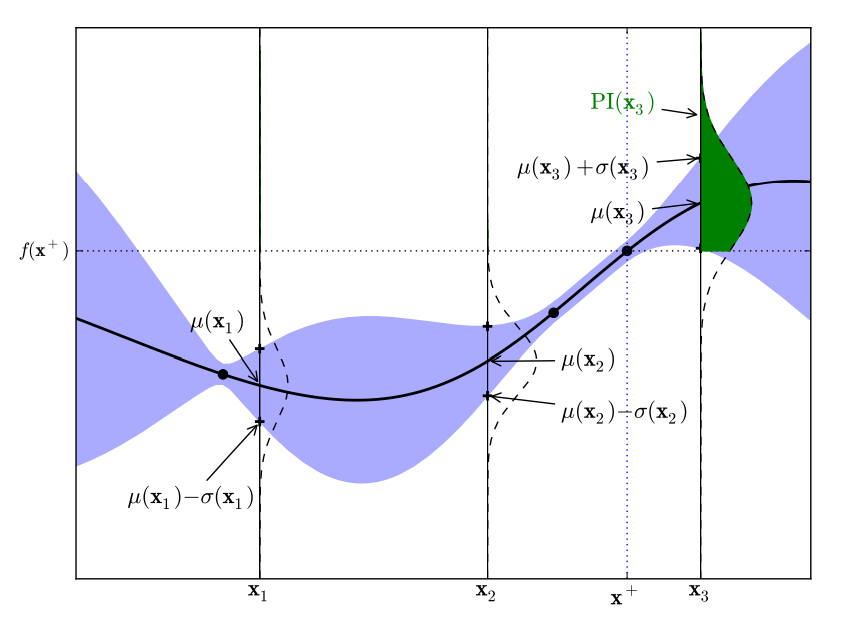
\includegraphics[scale=0.45]{imp.png}
\end{figure}
\end{center}
\end{frame}

\begin{frame}
\frametitle{Wybór jądra}
\begin{center}
\begin{figure}
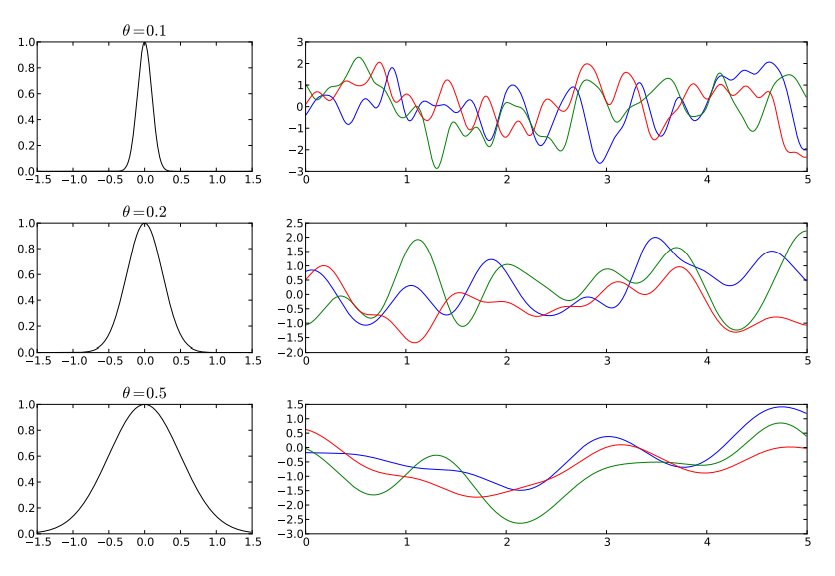
\includegraphics[scale=0.45]{kern.png}
\end{figure}
\end{center}
\end{frame}

\begin{frame}
	\frametitle{Bibliography}
	\begin{itemize}
	    \item Brochu E., Cora V. M., de Freitas N. (2010), A Tutorial on Bayesian Optimization of
Expensive Cost Functions, with Application to
Active User Modeling and Hierarchical
Reinforcement Learning,

		\item Bischl1 B., Wessing S., Bauer N., Friedrichs K., Weihs C., MOI-MBO: Multiobjective Infill for Parallel
Model-Based Optimization.
	\end{itemize}
\end{frame}



\end{document}